\section{Auswertung} 

\subsection{Geräteeinstellungen}

\begin{flushleft}
    Durchgeführt wurde ein A-Scan mittels des Impuls-Echo-Verfahrens der Acrylplatte.
    Als Koppelmittel wurde bidestiliertes Wasser benutzt.
    Aufgenommen wurden die Laufzeiten und die Amplituden, zu sehen in der Tabelle \ref{Tabelle2}.
    Die Acrylplatte hat eine Dicke von $s = 10\,\unit{\milli\meter}$.
    Die Schallgeschwindigkeit berechnet sich durch die Formel (\ref{6}).
\end{flushleft}

\begin{table}[H]
    \centering
    \caption{Laufzeiten und Amplituden} 
    \label{Tabelle2}
    \begin{tabular} {c  c}
        \toprule
        {$ \text{Laufzeiten}\, \text{t} \mathbin{/} \unit{\micro\second} $} &
        {$ \text{Amplituden}\, \text{t} \mathbin{/} \unit{\micro\second} $} \\
        \midrule
        7 & 0,5 \\
        7 & 0,5 \\
        7 & 0,6 \\
        8 & 0,5 \\
        7 & 0,6 \\
        \bottomrule
    \end{tabular} 
\end{table}

\begin{align}
    \intertext{Aus den Laufzeiten, mit $\overline{\text{T}} = (7,2 \pm 0,2)\,\unit{\micro\second}$, folgt für die Schallgeschwindigkeit }
    \text{c}_{\text{exp}} = ( 2777,7 \pm 158,8 )\,\frac{\unit{\meter}}{\unit{\second}}\,. \notag
    \intertext{Aus den Amplituden und somit der Frequenz leitet sich die Wellenlänge her, mit}
    \overline{\text{T}} = (0,54 \pm 0,04)\,\unit{\micro\second}\,, \notag \\
    \text{f} = \frac{1}{\text{T}} = (1,85 \pm 0,13) \cdot 10^{6}\,\unit{\hertz}\,, \label{7} \\
    \lambda = \frac{\text{c}_{\text{exp}}}{\text{f}} = (1,50 \pm 0,18) \cdot 10^{-3}\,\unit{\meter}\,. \label{8}
\end{align}

\begin{figure}[H]
    \centering
    \includegraphics[height=90mm]{bilder/GERÄTEEINST.1.2(neu).jpg}
    \caption{Impuls-Echo-Verfahren. \label{Abbildung1} }
\end{figure}

\begin{flushleft}
    Die Einstellungen wie AM, HF und $\text{AM}+\text{HF}$ verdeutlichen die Einhüllende sowie die Amplituden.
    Um die Amplituden zu untersuchen, ist es nötig, an jedem Tal die Grafik zu vergrößern.
\end{flushleft}

\subsection{Impuls-Echo-Verfahren} \label{sec:Kap5.2}

\begin{align*}
    \intertext{Für die Bestimmung der Schallgeschwindigkeit wurden folgende Abmessungen der Zylinder festgestellt}
    \text{ganz kleiner Zylinder}\,\,\,\,\, \text{l}_{\text{gk}} = 40,0175\,\unit{\milli\meter}\,, \\
    \text{kleiner Zylinder}\,\,\,\,\,\text{l}_{\text{k}} = 61,25\,\unit{\milli\meter}\,, \\
    \text{großer Zylinder}\,\,\,\,\, \text{l}_{\text{g}} = 80,25\,\unit{\milli\meter}\,, \\
    \text{ganz großer Zylinder}\,\,\,\,\, \text{l}_{\text{gg}} = 120,25\,\unit{\milli\meter}\,.
    \intertext{ In der Tabelle \ref{Tabelle3} sind für verschieden lange Zylinder mit dem A-Scan gemessenen Laufzeiten und Amplituden des ersten, welches als Theoriewert angenommen wird und zweiten Pulses aufgelistet. }
\end{align*}

\begin{table}[H]
    \centering
    \caption{Laufzeiten und Amplituden für das Impuls-Echo-Verfahren.} 
    \label{Tabelle3}
    \begin{tabular} {c  c  c  c  c}
        \toprule
        {$ \text{Länge der Zylinder}\, \text{l} \mathbin{/} \unit{\milli\meter} $} &
        {$ \text{t} \mathbin{/} \unit{\micro\second} $} &
        {$ \text{U} \mathbin{/} \unit{\volt} $} &
        {$ \text{t} \mathbin{/} \unit{\micro\second} $} &
        {$ \text{U} \mathbin{/} \unit{\volt} $} \\
        \midrule
        40,175 & 0 & 1,35 & 30 & 1,17 \\
        61,25  & 0 & 1,33 & 46 & 0,56 \\
        80,25  & 0 & 1,32 & 60 & 1,08 \\
        120,25 & 0 & 1,33 & 89 & 0,18 \\
        \bottomrule
    \end{tabular} 
\end{table}

\begin{align*}
    \intertext{Die Schallgeschwindigkeit kann nicht mit der Gleichung erfüllt werden, da systematische Fehler vorhanden sind.
    Deshalb wird eine Lineare Regression, mit der Funktion}
    \text{y} = \text{A\,x} + \text{B}
    \intertext{durchgeführt.
    Die Steigung entspricht der Schallgeschwindigkeit, der y-Achsenabschnitt der doppelten Dicke der Anpassungsschicht und deren Nullstelle der doppelten Laufzeit durch die Anpassungsschicht.}
\end{align*}

\begin{figure}[H]  
    \centering
    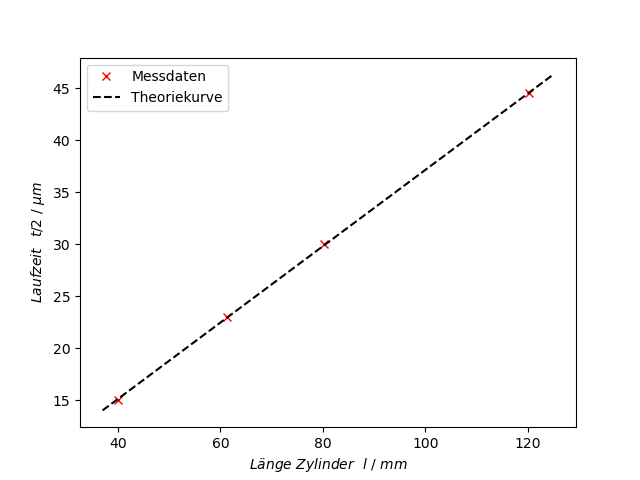
\includegraphics[height=80mm]{bilder/1.png}
    \caption{Lineare Regression beim Impuls-Echo-Verfahren. \label{Abbildung2} }
\end{figure}

\begin{align*}
    \intertext{Die Regression liefert die Werte}
    \text{Steigung $\text{A}_{\text{Echo}}$} = (2723,45 \pm 17,06)\,\frac{\unit{\meter}}{\unit{\second}}\,, \\
    \text{y - Achsenabschnitt $\text{B}_{\text{Echo}}$ } = (0,11 \pm 0,05)\,\unit{\centi\meter}\,, \\
    \text{d}_{\text{Echo}} = 0,055\,\unit{\centi\meter}\,, \\
    \text{t}_{\text{Anpassung, Echo}} = 0,022\,\unit{\micro\second}\,.
\end{align*}

\subsection{Dämpfung}

\begin{align}
    \intertext{Um die Dämpfung zu berechnen wird die Gleichung (\ref{4}) umgestellt zu}
    \alpha = - \frac{\ln\left(\frac{\text{U(x)}}{\text{U}_{0}}\right)}{\text{X}_{1}}\,. 
    \intertext{Dabei ist U(x) die Amplitude an der Stelle $\text{x}_{1} > 0 $ und $\text{U}_{0}$ die Amplitude an der Stelle $\text{x} = 0$.
    Angenommen wird der ganz kleine Zylinder mit den Messwerten }
    \text{l}_{\text{gk}} = 40,0175\,\unit{\milli\meter} = \text{x}_{1}\,, \notag \\
    \text{U}_{0} = 1,35\,\unit{\volt} \,\,\text{an der Stelle $\text{x} = 0$} \,, \notag \\
    \text{U(x)} = 1,17\,\unit{\volt}\,. \notag
    \intertext{Im Mittel ergibt sich die Dämpfungskonstante zu}
    \alpha = (3,57 \pm 0,26)\,\frac{1}{\unit{\meter}}\,. \notag
\end{align}

\subsection{Durchschallungs-Verfahren}

\begin{flushleft}
    Die Schallgeschwindigkeit wird eben sowie in Kapitel \ref{sec:Kap5.2} Impuls-Echo-Verfahren bestimmt, nur mit der Ausnahme, dass der Faktor $\frac{1}{2}$ wegfällt, da der Schall den Zylinder nur einmal durchläuft.
    Die Laufzeiten befinden sich in Tabelle \ref{Tabelle4}. 
    Erneut wird eine Lineare Regression durchgeführt.
\end{flushleft}

\begin{table}[H]
    \centering
    \caption{Laufzeiten und Amplituden beim Durchschallungs-Verfahren} 
    \label{Tabelle4}
    \begin{tabular} {c  c  c  c  c}
        \toprule
        {$ \text{Länge der Zylinder}\, \text{l} \mathbin{/} \unit{\milli\meter} $} &
        {$ \text{t} \mathbin{/} \unit{\micro\second} $} &
        {$ \text{U} \mathbin{/} \unit{\volt} $} &
        {$ \text{t} \mathbin{/} \unit{\micro\second} $} &
        {$ \text{U} \mathbin{/} \unit{\volt} $} \\
        \midrule
        40,175 & 0 & 1,33 & 15 & 0,72 \\
        61,25  & 0 & 1,33 & 23 & 0,47 \\
        80,25  & 0 & 1,33 & 31 & 0,29 \\
        120,25 & 0 & 1,34 & 45 & 0,03 \\
        \bottomrule
    \end{tabular} 
\end{table}

\begin{figure}[H]  
    \centering
    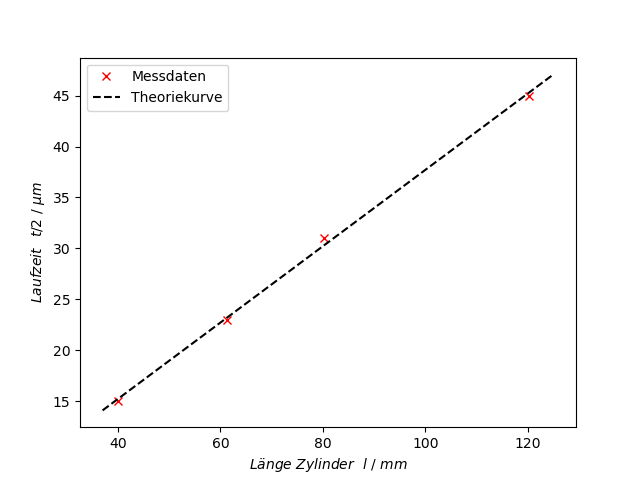
\includegraphics[height=80mm]{bilder/3.png}
    \caption{Lineare Regression beim Durchschallungs-Verfahren. \label{Abbildung4} }
\end{figure}

\begin{align*}
    \intertext{Die Parameter lauten}
    \text{A}_{\text{Durchschallung}} = (2663,21 \pm 68,87)\,\frac{\unit{\meter}}{\unit{\second}}\,, \\
    \text{B}_{\text{Durchschallung}} = (0,051 \pm 0,002)\,\unit{\centi\meter}\,, \\
    \text{d}_{\text{Durchschallung}} = 0,0255\,\unit{\centi\meter}\,, \\
    \text{t}_{\text{Durchschallung}} = 0,01\,\unit{\micro\second}\,.
\end{align*}

\subsection{Spektrale Analyse und Cepstrum}

\begin{flushleft}
    Zwei Acrylscheiben und ein $40\,\unit{\milli\meter}$ langer Zylinder werden aufeinander gelegt und mittels Wasser gekoppelt.
    Es werden Mehrfachimpulse im Impuls-Echo-Verfahren aufgenommen und mit Hilfe der FFT Funktion ein Spektrum und das Cepstrum der Sonde erzeugt.
    Aus dem Cepstrum der Ultraschallsonde, siehe Abbildung \ref{Abbildung5}, lassen sich drei Reflexionen erkennen, aus deren Laufzeiten berechnet sich die Dicke der Platten, mittels der Formel (\ref{6}).
\end{flushleft}

\begin{table}[H]
    \centering
    \caption{Berechnete Dicke der Scheiben.} 
    \label{Tabelle5}
    \begin{tabular} {c  c  c}
        \toprule
        {$  $} &
        {$ \text{t} \mathbin{/} \unit{\micro\second} $} &
        {$ \text{d} \mathbin{/} \unit{\milli\meter} $} \\
        \midrule
        Scheibe oben & 4,16 & 5,77 \\
        Scheibe unten & 7,44 & 10,33 \\
        Zusammen & 11,6 & 16,11 \\
        \bottomrule
    \end{tabular} 
\end{table}

\begin{figure}[H]
    \centering
    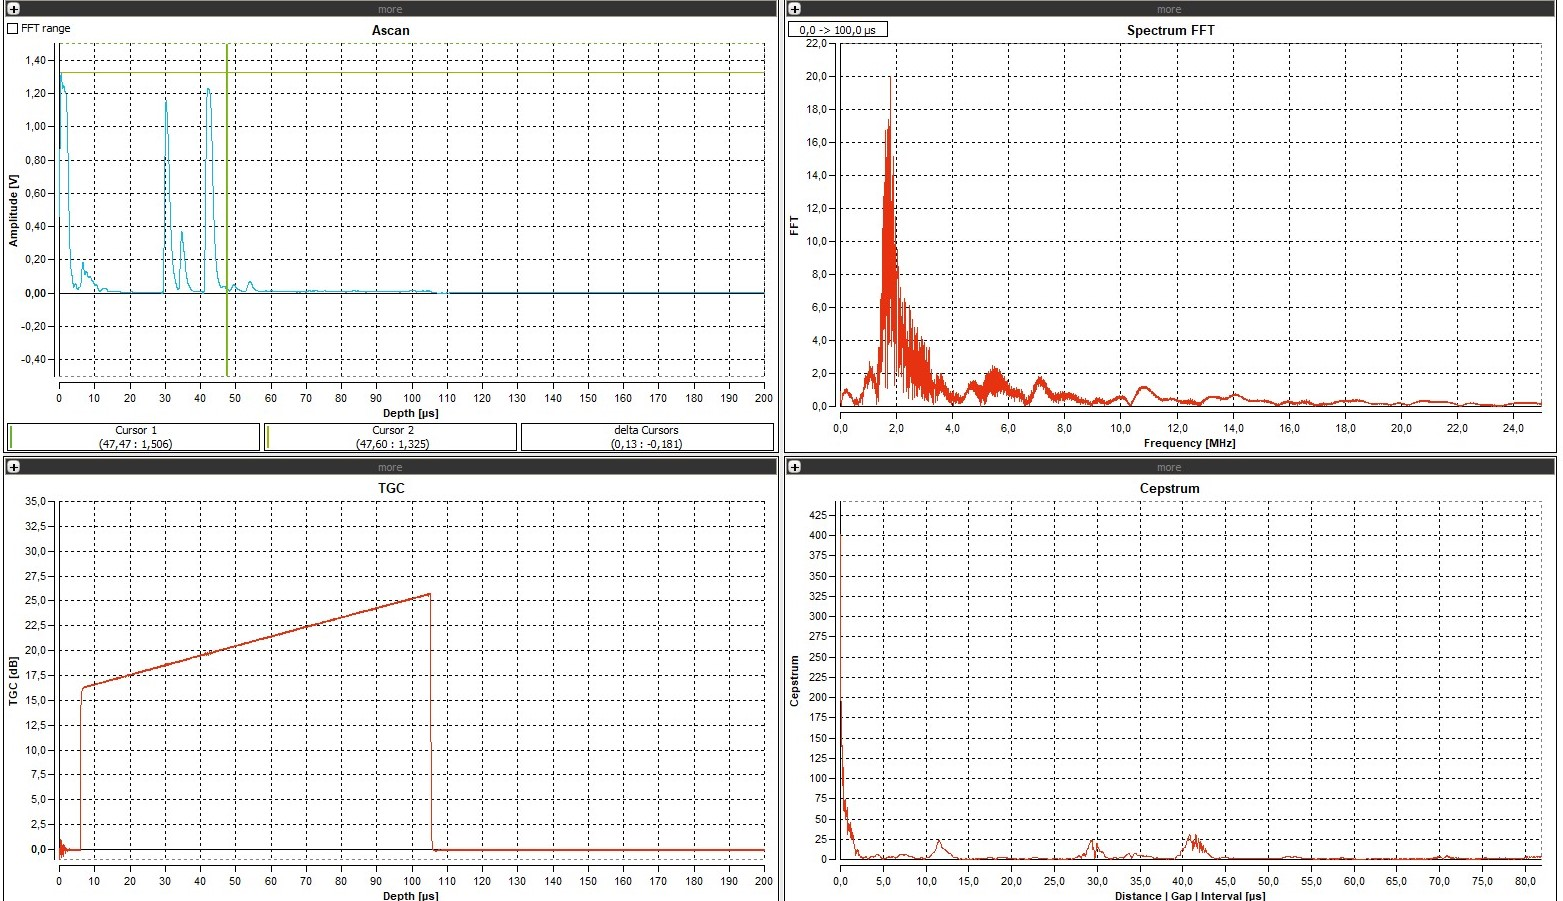
\includegraphics[height=80mm]{bilder/spektren.jpg}
    \caption{Spektrum der Ultraschallsonde. \label{Abbildung5} }
\end{figure}

\subsection{Abmessung des Auges}

\begin{flushleft}
    Im richtigen Einschallwinkel lassen sich vier Reflexionen im Auge messen, siehe Abbildung \ref{Abbildung6}, die die Grenzfläche der verschiedenen Augenbestandteile auftreten.
    Die Messwerte sind in der Tabelle \ref{Tabelle6} aufgelistet.
\end{flushleft}

\begin{table}[H]
    \centering
    \caption{Laufzeiten der Echos im Auge.} 
    \label{Tabelle6}
    \begin{tabular} {c  c  c  c}
        \toprule
        {$ \text{t}_{1} (\text{Hornhaut - Iris}) \mathbin{/} \unit{\micro\second} $} &
        {$ \text{t}_{2} (\text{Iris - Linse}) \mathbin{/} \unit{\micro\second} $} &
        {$ \text{t}_{3} (\text{Linse - Linse}) \mathbin{/} \unit{\micro\second} $} &
        {$ \text{t}_{4} (\text{Linse - Retina}) \mathbin{/} \unit{\micro\second} $} \\
        \midrule
        7 & 9 & 11 & 14 \\
        \bottomrule
    \end{tabular} 
\end{table}

\begin{flushleft}
    Es ist zu beachten, dass die Schallgeschwindigkeit in der Linse $\text{c}_{\text{L}} = 2500\,\frac{\unit{\meter}}{\unit{\second}}$ und in der Glaskörperflüssigkeit $\text{c}_{\text{K}} = 1410\,\frac{\unit{\meter}}{\unit{\second}}$ beträgt, sowie die Abstände voneinander abgezogen werden.
\end{flushleft}

\begin{table}[H]
    \centering
    \caption{Die Abmessungen des Augenmodels.} 
    \label{Tabelle7}
    \begin{tabular} {c  c  c  c}
        \toprule
        {$ \text{Hornhaut - Iris} \mathbin{/} \unit{\milli\meter}$} &
        {$ \text{Iris - Linse}    \mathbin{/} \unit{\milli\meter} $} &
        {$ \text{Linse - Linse}   \mathbin{/} \unit{\milli\meter} $} &
        {$ \text{Linse - Retina}  \mathbin{/} \unit{\milli\meter} $} \\
        \midrule
        4,6 & 2,2 & 6,95 & 16,82 \\
        \bottomrule
    \end{tabular} 
\end{table}

\begin{figure}[H]
    \centering
    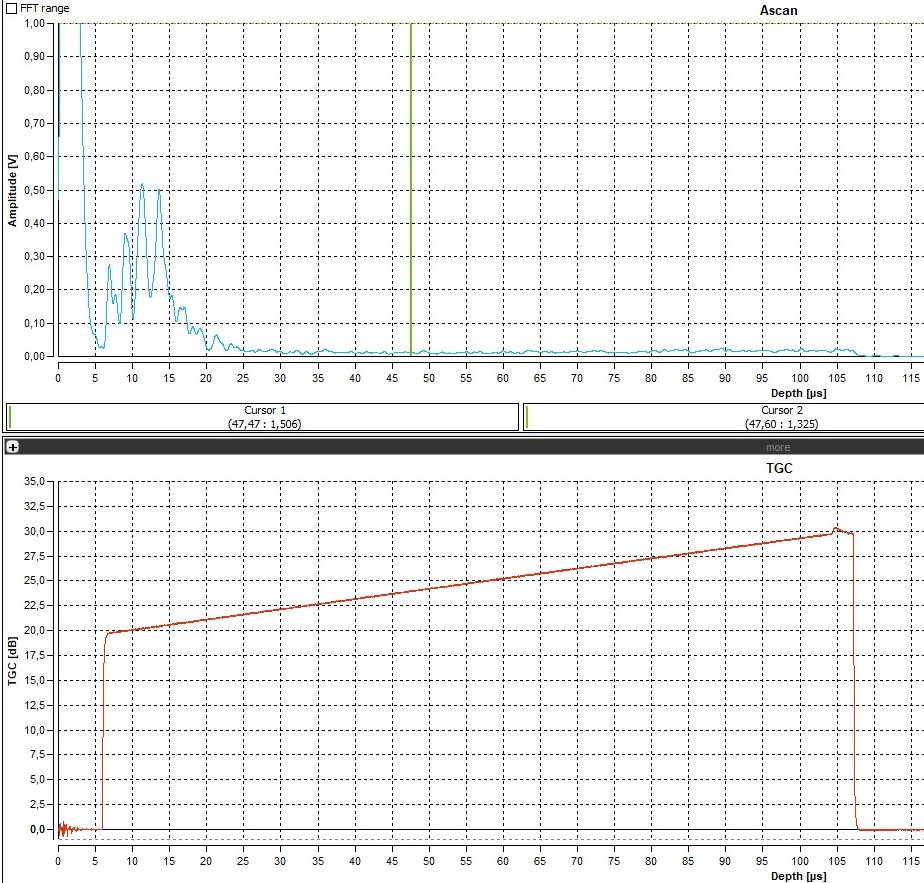
\includegraphics[height=80mm]{bilder/AUGE RICHTIG.jpg}
    \caption{Biometrische Untersuchung eines Augenmodells. \label{Abbildung6} }
\end{figure}